\documentclass[11pt]{article}
\usepackage{fullpage}
\usepackage{authblk}
\usepackage{graphicx}
\usepackage{subfig}
\usepackage{amsmath}
\usepackage{amsfonts}
\usepackage{amssymb}
\usepackage{amsthm}
\usepackage{mathrsfs}
\usepackage{enumitem}
\usepackage[ruled,vlined]{algorithm2e}

\newtheorem{theorem}{Theorem}[section]
\newtheorem{lemma}[theorem]{Lemma}
\newtheorem{claim}[theorem]{Claim}
\newtheorem{corollary}[theorem]{Corollary}
\newtheorem{proposition}[theorem]{Proposition}
\newtheorem{definition}[theorem]{Definition}
\newtheorem{remark}[theorem]{Remark}
\newtheorem{assumption}[theorem]{Assumption}
\newtheorem{hypothesis}[theorem]{Hypothesis}
\newtheorem{observation}[theorem]{Observation}

\makeatletter
\renewcommand\section{%
  \@startsection{section}{1}
                {\z@}%
                {-3.5ex \@plus -1ex \@minus -.2ex}%
                {2.3ex \@plus.2ex}%
                {\large\bfseries}% 11pt
}
\renewcommand\subsection{%
  \@startsection{subsection}{2}
                {\z@}%
                {-3.25ex\@plus -1ex \@minus -.2ex}%
                {1sp}% No space after subsections
                {\normalsize\bfseries}% normal size, boldface
}
\renewcommand\subsubsection{%
  \@startsection{subsubsection}{3}
                {\z@}%
                {-3.25ex\@plus -1ex \@minus -.2ex}%
                {1sp}% No space after subsubsections
                {\normalfont\normalsize}% normal size, medium
}
\makeatother
\marginparwidth 0pt \oddsidemargin 0pt \evensidemargin 0pt
\topmargin 30pt \textheight 21.0 truecm \textwidth 16.0 truecm

\title{\bf Packing Feedback Arc Sets in Reducible Flow Graphs}
\author{Han Xiao}

\affil{Department of Mathematics, The University of Hong Kong,

Hong Kong, China

{\tt hxiao.math@connect.hku.hk}}

\begin{document}
 \date{}
\maketitle
%\thispagestyle{empty}

\begin{abstract}
We establish a min-max relation in arc-weighted reducible flow graphs in this paper. In particular, we prove that the maximum cardinality of feedback arc set packings equals the minimum total weight of cycles.  We also present an $O(n^2 m)$ algorithm for finding a maximum feedback arc set packing in reducible flow graphs. Our result relies heavily on Ramachandran's \cite{Rama1,Rama2} structural analysis of reducible flow graphs.
\end{abstract}

\noindent{\bf Keywords.}\quad Min-max relation, feedback arc set, packing, reducible flow graph, algorithm


\openup 1.2\jot


\section{Introduction}
\label{intro}

A reducible flow graph is a special flow graph which corresponds to the flowchart of computer programs via structured programming. As described in \cite{Hech}, the ``divide-and-conquer'' approach applies to reducible flow graphs, which makes the analysis easier on such graphs. Reducible flow graphs also occur frequently in practice. Statistics suggest that most flow graphs associated with computer programs are reducible flow graphs. Therefore, reducible flow graphs have attracted many research efforts over the past few decades. Various characterizations of reducible flow graphs can be found in \cite{HecU1}. The first efficient algorithm for recognizing reducible flow graphs was given by Hopcroft and Ullman \cite{HopU}. Based on their work, Tarjan \cite{Tarj} derived a more efficient algorithm for testing flow graphs reducibility. 

As usual, by a cycle in a digraph we mean a directed one. A digraph is called \emph{acyclic} if it contains no cycles. Let $G=(V,A)$ be a digraph with a nonnegative integral function $w$ defined on arcs in $A$. A set $F\subseteq A$ is a \emph{feedback arc set} (FAS) for $G$ if $G^\prime=(V,A\backslash F)$ is acyclic. Let $H=(A,\mathcal{C})$ be a hypergraph whose vertex set is the arc set of $G$ and edges (with repetition allowed) are the arc sets of directed cycles in $G$. A subset $\mathcal{C}^\prime$ of edge set $\mathcal{C}$ in $H$ is called a \emph{cycle packing} if each arc $a\in A$ occurs at most $w(a)$ times in cycles of $\mathcal{C}^\prime$. A \emph{transversal} of a hypergraph is a subset of its vertex set which intersects each edge of the hypergraph. Note that a transversal of $H=(A,\mathcal{C})$ is a feedback arc set of $G$. Let $\nu_w$ denote the maximum cardinality of cycle packings and $\tau_w$ denote the minimum total weight of transversals. It is easy to prove that $\nu_w\leq\tau_w$. When equality $\nu_w=\tau_w$ holds for all nonnegative integral function $w$, the hypergraph $H$ is said to satisfy the min-max relation and the graph $G$ is said to be \emph{cycle Mengerian} (CM). In \cite{Rama1}, Ramachandran gave an $O(n^2m\log(n^2 / m))$ algorithm for finding a minimum weighted feedback arc set in arc-weighted reducible graphs. She \cite{Rama2} also established a conjecture of Frank and Gyarfas \cite{FraG} by proving that the cardinality of a minimum feedback arc set is equal to the cardinality of a maximum cycle packing  in unweighted reducible flow graphs. Her proof yielded an $O(\min\{mn^{5/3},m^2\})$ algorithm for finding a maximum collection of arc disjoint cycles. Chen and Zang \cite{CheZ} pointed out that although Ramachandran's proof \cite{Rama2} was intended for unweighted reducible flow graphs, it could be adapted to handle the weighted case. Based on Ramachandran's work \cite{Rama1,Rama2}, Chen and Zang proved that every reducible flow graph is CM. They also reduced the time complexity of finding a maximum cycle packing in weighted reducible flow graphs to $O(n^2 m\log(n^2/m))$  by avoiding using augmenting path method for finding the maximum flow as a subroutine in their algorithm. 

A \emph{clutter} is a hypergraph no edge of which is contained in another. Note that hypergraph $H=(A,\mathcal{C})$ is a clutter. The hypergraph $H^\perp=(A,\mathcal{F})$ is called the \emph{blocker} of $H$, if vertex set of $H^\perp$ is the arc set of $G$ and edges (with repetition allowed) are the collection of feedback arc sets. Analogous to the definition of cycle packing, we call a subset $\mathcal{F}^\prime$ of edge set $\mathcal{F}$ in $H^\perp$ a \emph{feedback arc set packing} if each arc $a$ occurs at most $w(a)$ times in feedback arc sets of $\mathcal{F}^\prime$. Note that a transversal of $H^\perp$ is a cycle in $G$. Let $\lambda_w$ denote the maximum cardinality of feedback arc set packings and $\mu_w$ denote the minimum total weight of transversals. Obviously, $\lambda_w\leq\mu_w$. When equality $\lambda_w=\mu_w$ holds for all nonnegative integral function $w$, the hypergraph $H^\perp$ is said to satisfy the min-max relation and the graph $G$ is said to be \emph{feedback arc set Mengerian} (FASM). It has been proved that hypergraph $H=(A,\mathcal{C})$ derived from reducible flow graph $G=(V,A)$ satisfies the min-max relation. Hence every reducible flow graph is CM. A natural question is whether the blocker $H^\perp=(A,\mathcal{F})$ of hypergraph $H$ satisfies the min-max relation as well. The main purpose of this paper is to give an affirmative answer to this question, i.e., every reducible flow graph is FASM. Moreover, we present an $O(n^2 m)$ algorithm for finding a maximum FAS packing in reducible flow graphs. Our result relies heavily on the structural analysis for reducible flow graphs of Ramachandran's work \cite{Rama1,Rama2}.

The remainder of this paper is organized as follows. In section 2, we introduce some preliminary knowledge on reducible flow graphs. In section 3, we first prove that every reducible flow graph is FASM, then we present our algorithm and establish its correctness.

\section{Preliminaries}
\label{prel}

A \emph{flow graph} is a digraph with a root such that the root reaches all other vertices via directed paths.
A \emph{DAG} is a directed acyclic graph. Let $G=(V,A;r)$ be a flow graph with root $r$. 
A \emph{DAG} of $G$ is a maximal acyclic subgraph of $G$ which remains a flow graph. We call $G$ \emph{reducible} if the DAG of $G$ is unique. A DAG of $G$ obtained from a depth-first spanning tree rooted at $r$ by adding a maximal subset of arc set $A$ is called a \emph{DFS DAG} of $G$.

For $u,v\in V$, we say $u$ \emph{dominates} $v$ if every $r-v$ path passes through $u$. Clearly, every vertex dominates itself. For a subgraph $G'$ of $G$, a vertex $v$ of $G'$ is called an \emph{entry vertex} if $v=r$ or there is an arc $(u,v)$ of $G$ with $u$ outside $G'$.  Observe that arcs in a reducible flow graph can be uniquely partitioned into the \emph{forward} (or \emph{DAG}) \emph{arc} set and the \emph{back arc} set.

Following are some useful characterizations of reducible flow graphs.
\begin{theorem}
\label{thm:1}
Let $G=(V,A;r)$ be a flow graph and let $D$ be a DFS DAG of $G$. Then the following statements are equivalent:
\begin{enumerate}[label=\emph{(}\alph*\emph{)}]
  \item $G$ is a reducible flow graph.
  \item $F$ is a forbidden structure of $G$ (see Figure \ref{fig:1}).
  \item $D$ is the unique DAG of $G$.
  \item The arc set $A$ can be partitioned into $A_1$ and $A_2$ such that $(V,A_1;r)$ is a DAG of $G$ and $u$ dominates $v$ in $G$ for each arc $(v,u)$ in $A_2$.
  \item Every cycle $C$ in $G$ contains exactly one back arc $a\in A\backslash A(D)$. Moreover, the head of back arc $a\in A\backslash A(D)$ is the entry vertex of $C$ which dominates other vertices on $C$.
\end{enumerate}
\end{theorem}

\begin{figure}
\centering
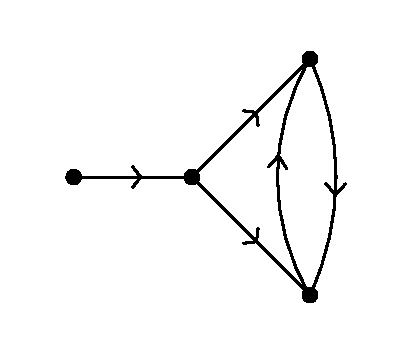
\includegraphics{FASPacking-fig1.eps}
\caption{The forbidden subgraph $F$}
\label{fig:1}
\end{figure}

\begin{proof}
The equivalence of $(a)-(d)$ can be found in \cite{HecU1} and \cite{HecU2}. The implication $(a)\Rightarrow (e)$ is proved in \cite{Sham} and the converse direction $(e)\Rightarrow (a)$ is contained in \cite{CheZ}.
\end{proof}

Throughout this paper, we use $V_h$ to denote the set of heads of all back arcs in $G$, $T_h$ to denote the \emph{head dominator tree} of $G$ which demonstrates the domination relation on $V_h\cup \{r\}$: the descendants of a vertex $u$ in $T_h$ are precisely the vertices in $V_h$ dominated by $u$ in $G$. For each $u\in V_h\cup\{r\}$, let $(u_1,v_1)$, $(u_2,v_2)$,\dots,$(u_k,v_k)$ be all the back arcs in $G$ whose heads are dominated by $u$. We use $V_u$ to denote the \emph{dominated back arc vertex set} of $u$ which consists of all the vertices in $V$ lying on some DAG path from $u$ to $u_i$, for $1\leq i\leq k$. Ramachandran \cite{Rama1,Rama2} proved that $u$ dominates all vertices in $V_u$. Let $G_s(V_u)$ be the subgraph of $G$ induced by $V_u$ (see Figure \ref{fig:2}).

\begin{figure}
    \centering
    \subfloat[$G$]{
    \begin{minipage}[t]{0.33\linewidth}
          \centering
          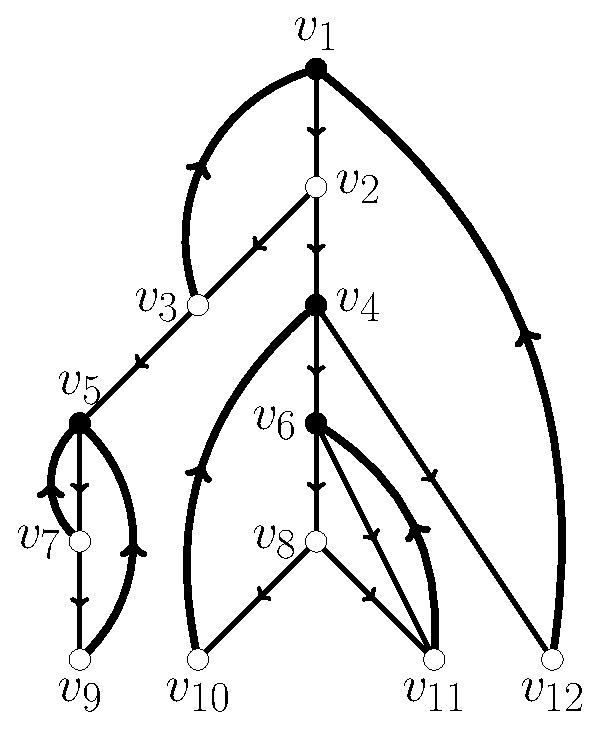
\includegraphics[scale=.45]{FASPacking-fig2a.eps}
          \label{fig:2a}
    \end{minipage}}
    \subfloat[$T_h$]{
     \begin{minipage}[t]{0.33\linewidth} 
          \centering
          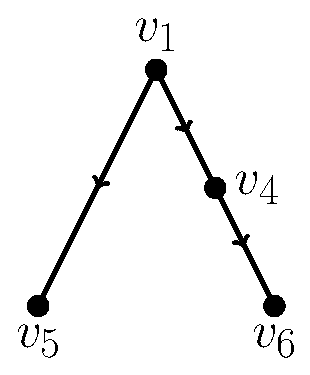
\includegraphics[scale=.45]{FASPacking-fig2b.eps}
          \label{fig:2b}
    \end{minipage}}
    \subfloat[$G_s(V_{v_4})$]{
    \begin{minipage}[t]{0.33\linewidth} 
          \centering
          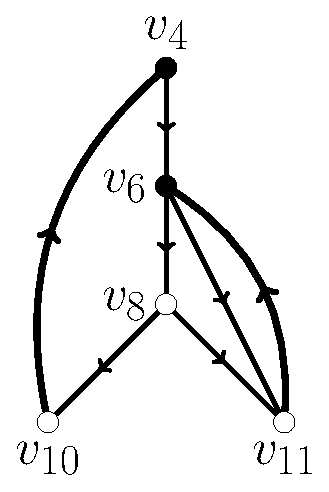
\includegraphics[scale=.45]{FASPacking-fig2c.eps}
          \label{fig:2c}
    \end{minipage}}  
    \caption{Reducible flow graph $G$ and corresponding $T_h$, $G_s(V_{v_4})$}
     \label{fig:2}
 \end{figure}

The following properties on dominated back arc vertex sets were established by Chen and Zang \cite{CheZ}.

\begin{theorem}
\label{thm:2}
Let $G=(V,A;r)$ be a reducible flow graph and let $u$, $v$ be two vertices in $V_h\cup\{r\}$. Then the following statements hold:
\begin{enumerate}[label=\emph{(}\alph*\emph{)}]
  \item $G_s(V_u)$ is a reducible flow graph rooted at $u$.
  \item $u$ is the unique entry vertex of $G_s(V_u)$ in $G$.
  \item If $G_s(V_u)$ and $G_s(V_v)$ have a common vertex, then either $u$ dominates $v$ or $v$ dominates $u$.
\end{enumerate}
\end{theorem}

Let $G=(V,A)$ be a digraph with a nonnegative length $l(a)$ on each arc $a\in A$. For each path $P=(v_0,a_1,v_1,\dots,a_m,v_m)$, the \emph{length} $l(P)$ is defined by:
\begin{equation*}
l(P):=\sum_{i=1}^m l(a_i).
\end{equation*}

Let $s,t$ be two vertices in $V$. The \emph{distance} from $s$ to $t$ (with respect to $l$), denoted by $d(s,t)$, is equal to the minimum length of all $s-t$ paths. If no $s-t$ path exists, $d(s,t)$ is set to $+\infty$.

The following theorem is due to Robacker \cite{Roba}. Since the proof technique plays an important role in this paper, for completeness we include Robacker's proof here.
\begin{theorem}
\label{thm:3}
Let $G=(V,A)$ be a digraph, $s,t\in V$ and let $l:A\rightarrow \mathbb{Z}_+$. Then the minimum length of an $s-t$ path is equal to the maximum size $k$ of a family of $s-t$ cuts $C_1,C_2,\dots,C_k$ (with repetition allowed) such that each arc $a$ is in at most $l(a)$ of the cuts $C_i$.
\end{theorem}
\begin{proof}
Note that if $P$ is any $s-t$ path and $C_1,C_2,\dots,C_k$ is any collection as described in the theorem, then
\begin{equation*}
\begin{split}
&~ l(P)=\sum_{a\in A(P)}l(a)\geq \sum_{a\in A(P)}(\mbox{number of $i$ with $a\in C_i$})\\
&=\sum_{i=1}^k\lvert C_i\cap A(P)\rvert \geq \sum_{i=1}^k 1=k.
\end{split}
\end{equation*}
So the minimum is bounded from below by maximum. To establish equality, let $d$ be the distance from $s$ to $t$, and let $U_i$ be the set of vertices at distance less than $i$ from $s$, for $i=1,\dots,d$. Taking $C_i:=\partial^+(U_i)$, we obtain a collection $C_1,C_2,\dots,C_d$ as required.
\end{proof}


\section{Maximum feedback arc set packings in reducible flow graphs}
\label{sec:3}

\subsection{Min-max relation}
\label{sec:4}

Let $G=(V,A;r)$ be a reducible flow graph with a nonnegative integral weight $w(a)$ on each arc $a\in A$. For each $u\in V_h\cup\{r\}$, we construct a network $N(u,t)$ from $G_s(V_u)$ as follows. Split every head $v$ in $G_s(V_u)\cap V_h$ into two vertices $v$ and $v^\prime$ and add a new vertex $t$. For all arcs incident to the original head $v$ (both entering and leaving $v$), connect all DAG arcs to the vertex $v$ in $N$ in the same manner as the original arcs in $G_s(V_u)$ (entering arcs remain entering arcs, and leaving arcs remain leaving arcs) and connect all back arcs to the vertex $v^\prime$ in $N$ also in the same manner as the original arcs in $G_s(V_u)$. Besides, connect every $v^\prime$ to $t$ by a \emph{newly added arc} $(v^\prime,t)$. 

\begin{figure}
    \centering
    \subfloat[$N(v_1,t)$]{
    \begin{minipage}[t]{0.5\linewidth}
          \centering
          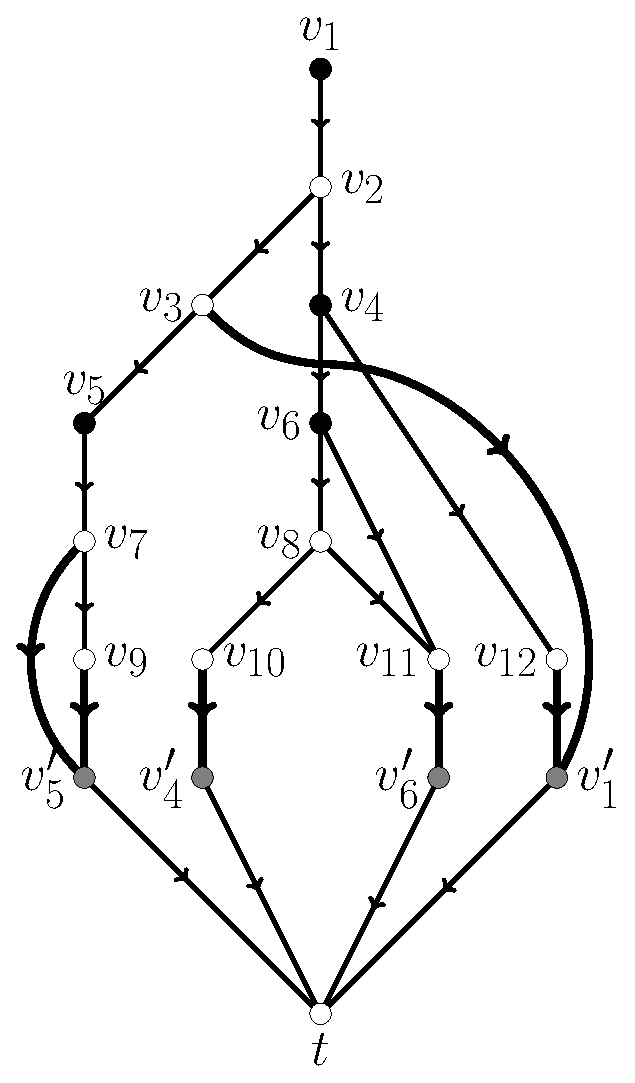
\includegraphics[scale=.425]{FASPacking-fig3a.eps}
          \label{fig:3a}
    \end{minipage}}
    \subfloat[$N(v_4,t)$]{
     \begin{minipage}[t]{0.5\linewidth} 
          \centering
          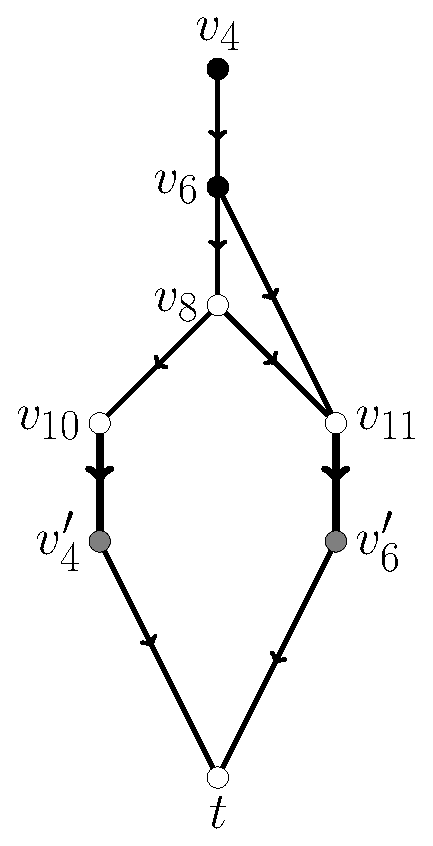
\includegraphics[scale=.425]{FASPacking-fig3b.eps}
          \label{fig:3b}
    \end{minipage}} 
    \caption{Network $N(v_1,t)$ and $N(v_4,t)$ obtained from reducible flow graph $G$}
     \label{fig:3}
 \end{figure}

\begin{lemma}
\label{lem:1}
Let $u,v\in V_h\cup\{r\}$. Then
\begin{enumerate}[label=\emph{(}\alph*\emph{)}]
  \item $u^\prime$ is not contained in $N(v,t)$ while $v^\prime$ is contained in $N(u,t)$ iff $u$ dominates $v$.
  \item Either $N(u,t)\backslash\{t\}$ and $N(v,t)\backslash\{t\}$ are vertex disjoint or one of $N(u,t)$ and $N(v,t)$ is contained in the other.
  \item $N(u,t)$ is an acyclic digraph rooted at $u$.
\end{enumerate}
\end{lemma}
\begin{proof}
Note that $u^\prime$ is not contained in $N(v,t)$ and $v^\prime$ is contained in $N(u,t)$ iff $u\not\in V_v$ and $v\in V_u$ iff $u$ dominates $v$. So $(a)$ follows.

Suppose $N(u,t)\backslash\{t\}$ and $N(v,t)\backslash\{t\}$ have a vertex in common. From their construction, we deduce that $G_s(V_u)$ and $G_s(V_v)$ have the same common vertex. By Theorem \ref{thm:2}, $u$ dominates $v$ or $v$ dominates $u$. Without loss of generality, we may assume that $u$ dominates $v$. Then $V_v\subseteq V_u$. Again from the construction, $N(v,t)$ must be contained in $N(u,t)$.

By Theorem \ref{thm:2}, $G_s(V_u)$ is a reducible flow graph rooted at $u$. And in the construction of $N(u,t)$ from $G_s(V_u)$, we break all cycles in $G_s(V_u)$. So $(c)$ follows.
\end{proof}

In the following, we focus on network $N(r,t)$ and denote it by $N$ for short. We extend the weight function $w$ on arcs in $G=(V,A;r)$ to a length function $l$ on arcs in $N$: first, set $l(a)=w(a^\prime)$ for each arc $a\in A(N)$ that corresponds to arc $a^\prime\in A$; then, for each newly added arc $a=(v^\prime,t)$ in $A(N)$, set $l(a)=d-d(v)$, where $d(v)$ is the distance from $r$ to $v$ in $N$ and $d:=\max_{v\in V_h} d(v)$ stands for the largest distance from $r$ to every vertex in $V_h$. Obviously, $l(a)\geq 0$ for all $a\in A(N)$. We denote the arc weighted network by $N(r,t;l)$. In network $N(r,t;l)$, the set of all vertices at distance less than $i$ from $r$ is denoted by $U_i$ and the set of all outgoing arcs of set $U_i$ is denoted by $\partial^+(U_i)$.

\begin{lemma}
\label{lem:2}
For each $v\in V_h$, the following statements hold:
\begin{enumerate}[label=\emph{(}\alph*\emph{)}]
  \item There is a one to one correspondence between cycles whose head of back arc is $v$ in $G$ and $v-t$ paths passing through $v^\prime$ in $N$. 
  \item Among all $r-t$ paths in $N$ passing through $v^\prime$, the shortest length is $d+d(v,v^\prime)$.
\end{enumerate}
\end{lemma}
\begin{proof}
From the construction of $N$, $(a)$ follows directly.

By Theorem \ref{thm:2}, $v$ is the only entry vertex of $G_s(V_v)$. From the construction, we see that $v$ is the only entry vertex of $N(v,t)\backslash\{t\}$. Since any part of the shortest path is also a shortest path, so the length of the shortest $r-t$ paths passing through $v^\prime$ is $d(v)+d(v,v^\prime)+d(v^\prime,t)=d(v)+d(v,v^\prime)+d-d(v)=d+d(v,v^\prime)$.
\end{proof}

Let $K$ denote the minimum total weight of cycles in $G$ throughout this paper. By Lemma \ref{lem:2}, $d(t)=\min_{v\in V_h}\{d+d(v,v^\prime)\}=d+K$, implying that the total number of $r-t$ cuts $\partial^+(U_i)$ in $N$ is $d+K$.

Inspired by the proof of Theorem \ref{thm:3}, if deleting $r-t$ cut $\partial^+(U_i)$ breaks all $v-v^\prime$ paths in $N(r,t;l)$ for every $v\in V_h$, then $\partial^+(U_i)$ naturally yields an FAS in $G=(V,A;r)$, and all such sets form an FAS packing of $G$. Unfortunately, we cannot even guarantee the existence of such $\partial^+(U_i)$ in $N(r,t;l)$, not to mention maximizing the collection of such sets. However, the hierarchy structure of network $N(r,t;l)$ inherited from reducible flow graphs enables us to tackle this question in an augmenting way: when necessary, we use more than one $r-t$ cuts $\partial^+(U_i)$ from $N$ to form an FAS of $G$ and manage to maximize the number of FAS we can get.

By Theorem \ref{thm:1}, each cycle in reducible flow graph $G$ contains a unique back arc. We may decompose all the cycles in $G$ into disjoint subsets according to their back arcs. However, different back arcs may share the same head and cycles whose back arcs sharing the same head do not make any differences for us in this paper, so we give the decomposition by heads of back arcs. Let $C_v$ be the collection of all cycles in $G$ whose head of back arc is $v\in V_h$. We call $\partial^+(U_i)$ in $N$ a \emph{quasi} cut of $C_v$ if deleting $\partial^+(U_i)$ breaks all $v-t$ paths in $N$, a \emph{proper} cut of $C_v$ if deleting $\partial^+(U_i)$ breaks all $v-v^\prime$ paths in $N$. Let $\mathcal{C}$ be the collection of $C_v$ in $G$ for some $v\in V_h$. We call $\partial^+(U_i)$ in $N$ a \emph{quasi} cut of $\mathcal{C}$ if $\partial^+(U_i)$ is a quasi cut for every $C_v\in\mathcal{C}$. Besides, we call a quasi cut $\partial^+(U_i)$ of $\mathcal{C}$ a \emph{quasi} FAS of $G$ if $\mathcal{C}$ is the collection of $C_v$ for every $v\in V_h$. By Lemma \ref{lem:2}, it is easy to see that $\partial^+(U_i)$ is a quasi cut of $C_v$ if $d(v) <i\leq d(t)$, a proper cut of $C_v$ if $d(v)<i\leq \min\{d(t),d(v^\prime)\}$, a quasi cut of $\mathcal{C}$ if $\max_{v:C_v\in \mathcal{C}}d(v)<i\leq d(t)$ and a quasi FAS of $G$ if $d<i\leq d(t)$. Furthermore, for $v\in V_h$, the number of quasi cuts of $C_v$ is $d(t)-d(v)$ and the number of proper cuts of $C_v$ is $\min\{d(t),d(v^\prime)\}-d(v)$; for a collection $\mathcal{C}$ of $C_v$, the number of quasi cuts of $\mathcal{C}$ is $d(t)-\max_{v:C_v\in \mathcal{C}}d(v)$; the number of quasi FASs of $G$ is $d(t)-d=K$.

We are interested in distinguishing these $r-t$ cuts $\partial^+(U_i)$ because starting with a quasi FAS $\partial^+(U_i)$ of $G$, we can construct a valid FAS by attaching some quasi cuts of a series of nested subsets of $\mathcal{C}$, where $\mathcal{C}$ is the collection of all $C_v$ such that $(v^\prime,t)\in \partial^+(U_i)$. Furthermore, it turns out that we can achieve the maximum number of valid FASs in such a manner.

Now let us see how to construct a valid FAS of $G$ from a quasi FAS $\partial^+(U_i)$ so that we can maximize the number of valid FASs. If a quasi FAS $\partial^+(U_i)$ contains no newly added arc $(v^\prime,t)$, then replace each arc in $\partial^+(U_i)$ by its corresponding arc in $G$, which directly yields a valid FAS of $G$. So assume there are newly added arcs $(v^\prime,t)$ in quasi FAS $\partial^+(U_i)$ and let $\mathcal{C}$ be the collection of all $C_v$ associated with those newly added arcs. Note that it is the newly added arcs in quasi FAS $\partial^+(U_i)$ or equivalently the collection $\mathcal{C}$ that prevents $\partial^+(U_i)$ from being a valid FAS. To construct a valid FAS, we need to cut off all $v-v^\prime$ paths for each $C_v\in\mathcal{C}$. A straightforward idea is to attach a proper cut of $C_v$ to the initial quasi FAS $\partial^+(U_i)$ for each $C_v\in \mathcal{C}$. As we shall see, the first available\footnote{`First available' here refers to the $r-t$ cut $\partial^+(U_i)$ with the least index $i$ among all unused cuts.} quasi cut of $\mathcal{C}$ is always an available proper cut of some $C_v\in\mathcal{C}$ throughout our construction process, which serves the purpose very well. In the following, we say $r-t$ cut $\partial^+(U_i)$ in $N$ \emph{breaks} $C_v$ if $\partial^+(U_i)$ is a proper cut of $C_v$. When $\mathcal{C}$ is not empty, we recursively choose the first available quasi cut of current $\mathcal{C}$ as a supplement of the initial quasi FAS $\partial^+(U_i)$ and delete every $C_v$ from $\mathcal{C}$ that is broken by this quasi cut. We call an execution of choosing the first available quasi cut of current $\mathcal{C}$ and deleting the broken cycle classes from $\mathcal{C}$ an \emph{iteration}. As long as we have available quasi cuts breaking some $C_v\in\mathcal{C}$ in each iteration before $\mathcal{C}$ becomes empty, the cardinality of $\mathcal{C}$ decreases by at least one in each iteration and we will finally arrive at a valid FAS of $G$: when $\mathcal{C}$ is empty, take the union of the initial quasi FAS and all the chosen quasi cuts, delete all newly added arcs from its union and replace each arc by its corresponding arc in $G$. For simplicity, we call the process of constructing a valid FAS a \emph{stage}.

Observe that the initial quasi FAS of each stage is actually the first available quasi cut of $\mathcal{C}$, where $\mathcal{C}$ is the collection of $C_v$ for every $v\in V_h$. Therefore our construction process in each stage has a slightly different interpretation. Instead of starting with a quasi FAS, we start with an empty set $F$ and initialize $\mathcal{C}$ by the collection of $C_v$ for every $v\in V_h$. When $\mathcal{C}$ is not empty, we recursively choose the first available quasi cut $\partial^+(U_i)$ of current $\mathcal{C}$, merge $\partial^+(U_i)$ into $F$, and update $\mathcal{C}$ by deleting every $C_v$ that is broken by $\partial^+(U_i)$. When $\mathcal{C}$ becomes empty, the resulting $F$ breaks all $C_v$ for every $v\in V_h$. Deleting all newly added arcs in $F$ and replacing each arc in $F$ by its corresponding arc in $G$ give rise to a valid FAS of $G$.

Now the problem boils down to showing that in the construction of each stage, the first available quasi cut of current $\mathcal{C}$ always breaks some $C_v\in\mathcal{C}$ before $\mathcal{C}$ becomes empty. Notice that in the worst case, we need a proper cut for every $C_v\in\mathcal{C}$. Therefore if we can show that we always have enough available proper cuts for every $C_v\in \mathcal{C}$ throughout the construction process, we are done. The following lemma guarantees that we always have enough available proper cuts of $C_v$ for every $v\in V_h$ and hence iterations always end in each stage.

\begin{lemma} 
\label{lem:3}
Let $\mathcal{C}$ be the collection of $C_v$ for every $v\in V_h$. At each stage, if we initially start with $\mathcal{C}$, recursively choose the first available quasi cut of $\mathcal{C}$ in $N(r,t;l)$ and delete every cycle class $C_v$ that is broken by this quasi cut from $\mathcal{C}$, then we always end up with an empty set $\mathcal{C}$. Moreover, at the end of stage $k$, the number of available proper cuts of $C_v$ for each $v\in V_h$ is at least $K-k$.
\end{lemma}

Our proof of Lemma \ref{lem:3} is based on the following technical lemma. 

\begin{lemma}
\label{lem:4} 
In each iteration of a stage, let $\mathcal{C}^\prime\subseteq\mathcal{C}$ be the collection of all cycle classes in $\mathcal{C}$ such that the first available quasi cut $\partial^+(U_i)$ of current $\mathcal{C}$ is also the first available proper cut for each cycle class in $\mathcal{C}^\prime$. If $\mathcal{C}^\prime$ is not empty, then there exists a cycle class $C_u\in \mathcal{C}^\prime$ such that the number of available proper cuts of $C_u$ is decreased by precisely one in this stage.
\end{lemma}

\begin{proof}
Assume to the contrary that the number of available proper cuts of each cycle class in $\mathcal{C}^\prime$ is decreased by more than one in this stage. Since after this iteration, all cycle classes in $\mathcal{C}^\prime$ will be deleted from $\mathcal{C}$. Therefore no proper cuts of each cycle class in $\mathcal{C}^\prime$ will be chosen in the succeeding iterations of this stage. It follows that all other proper cuts of each cycle class in $\mathcal{C}^\prime$ are chosen before this iteration. However, in this case, $\partial^+(U_i)$ is no longer the first available quasi cut of $\mathcal{C}$ as all cycle classes in $\mathcal{C}^\prime$ are deleted from $\mathcal{C}$ before this iteration and the first available quasi cut of $\mathcal{C}$ will not depend on them, a contradiction.
\end{proof}

Notice that each $r-t$ cut $\partial^+(U_i)$ of $N$ can only be used once in constructing the collection of FAS. Therefore, at the end of each stage, we go through every $r-t$ cut $\partial^+(U_i)$ in $N$ and decrease the value of $l(a)$ by one for each arc $a\in \partial^+(U_i)$ if $\partial^+(U_i)$ is a chosen quasi cut at this stage. As a result, the constantly updated length function $l$ and the latest distance $d(v)$ for $v\in V(N)$ provide some useful information in every repetition of stages: for each $v\in V_h$, the difference $\min\{d(t),d(v^\prime)\}-d(v)$ is exactly the number of currently available proper cuts of $C_v$. Besides, the first available quasi cut of current $\mathcal{C}$ in each iteration of a stage is exactly the first cut of $C_v$ with the largest $d(v)$ in $\mathcal{C}$.

Now we are ready to present a proof of our key lemma.

\begin{proof}[Proof of Lemma \ref{lem:3}]
We apply induction on the number of stages.

Observe that the initial state, viewed as stage 0, automatically satisfies the induction hypothesis. Therefore, the proof of basis and the proof of induction step are essentially the same. So we proceed to the induction step. Suppose the statement in Lemma \ref{lem:3} holds for stage $k\geq 0$. We aim to establish the statement for stage $k+1$.

We initially start with $\mathcal{C}$ which consists of $C_v$ for every $v\in V_h$. By induction hypothesis, at the beginning of stage $k+1$, the number of available proper cut of $C_v$ for every $v\in V_h$ is at least $K-k>0$. Therefore, every $C_v$ for $v\in V_h$ has available proper cuts. Let $C_u$ be an arbitrary cycle class in $\mathcal{C}$. Let $\partial^+(U_{i_\tau}),\dots,\partial^+(U_{i_1})$ with $i_\tau<\dots<i_1$ be all the proper cuts of $C_u$ used in stage $k+1$. Assume these $r-t$ cuts are chosen as the first available quasi cut of a series of nested subsets $\mathcal{C}^{(\tau)}\subset\dots\subset\mathcal{C}^{(1)}:=\mathcal{C}$ respectively. If $\tau=1$, the number of available proper cuts of $C_u$ decreases by one. By induction hypothesis, the number of available proper cuts of $C_u$ is at least $K-k-1$ at the end of stage $k+1$. So assume $\tau\geq 2$. Let $u_j\in V_h$ be a vertex with the largest $d(v)$ among all $C_v\in \mathcal{C}^{(j)}$ for $j=\tau,\dots,1$. Since every $C_v$ for $v\in V_h$ has available proper cuts, the first available quasi cut $\partial^+(U_{i_j})$ of $\mathcal{C}^{(j)}$ is essentially the first available proper cut of $C_{u_j}\in \mathcal{C}^{(j)}$. Without loss of generality, assume $C_{u_j}$ is a cycle class in $\mathcal{C}^{(j)}$ whose number of available proper cuts decreases by one in this stage. By Lemma \ref{lem:4}, such $C_{u_j}$ exists. It follows that $d(u)\leq d(u_\tau)< d(u^\prime_\tau)\leq\dots\leq d(u_1)< \min\{d(t),d(u^\prime)\}$. Obviously, $C_u$ is not the cycle class with the least number available proper cuts among all vertices in $V_h$, since $\min\{d(t),d(u^\prime)\}-d(u)> d(u_\tau^\prime)-d(u_\tau)$. Moreover, by Lemma \ref{lem:4}, the number of available proper cuts of $C_{u_\tau}$ decreases by one in this stage. Then inequality $\min\{d(t),d(u^\prime)\}-d(u)>d(u_\tau^\prime)-d(u_\tau)$ together with the induction hypothesis implies that the number of available proper cuts of $C_u$ decreases by $\tau\geq 2$, but is no less than $K-k-1$ at the end of stage $k+1$.

Therefore, we always have available proper cuts of $C_v$ for every $v\in V_h$ in each iteration of a stage. So the first available quasi cut of current $\mathcal{C}$ is also the first available proper cut of some $C_v\in \mathcal{C}$. As a result, the cardinality of $\mathcal{C}$ decreases in each iteration. We finally arrive at an empty set $\mathcal{C}$ and hence iterations end in each stage.
\end{proof}

Recall that there are $K$ quasi FASs in $N$, and we only use one quasi FAS in a stage. As a result, there will be $K$ stages throughout the construction process. Moreover, Lemma \ref{lem:3} guarantees each stage returns a valid FAS of $G$. Therefore we can attain an FAS packing of cardinality $K$. Since $K$ is also the minimum total weight of cycles in $G$, the following theorem follows directly.

\begin{theorem}
\label{thm:4}
Every reducible flow graph is FASM.
\end{theorem}

\subsection{Algorithm and complexity}
\label{sec:5}
The constructive proof given above naturally yields an algorithm for finding a maximum FAS packing in a reducible flow graph $G$. However, regardless of other operations, we still need to repeat stage $K$ times before we arrive at a maximum FAS packing, which makes our algorithm pseudo-polynomial. Fortunately, consecutive stages might return the same valid FAS because those chosen proper quasi cuts in each stage might be the same. So a natural idea is to merge these consecutive stages returning the same valid FAS into one new stage.  
Suppose we have merged the first $k-1$ stages returning the same valid FAS into $\kappa-1$ new STAGEs respectively and updated the length function $l$ accordingly. Now we are at stage $k$, which cannot be merged into STAGE $\kappa-1$. We start our construction with $\mathcal{C}$ which initially consists of $C_v$ for every $v\in V_h$. Then we recursively choose the first available quasi cut of current $\mathcal{C}$ in $N$, delete every cycle class $C_v$ from $\mathcal{C}$ that is broken by the chosen quasi cut, and update $d$ by $\max_{C_v\in\mathcal{C}} d(v)$. After $j\geq 0$ iterations, we arrive at a nonempty set $\mathcal{C}$, and $\partial^+(U_{d+1})$ is the first available quasi cut of current $\mathcal{C}$. Observe that the following $\min_{(u,w)\in\partial^+(U_{d+1})}\{d(w)-d\}$ quasi cuts of current $\mathcal{C}$ including $\partial^+(U_{d+1})$ are actually the same. If current $\mathcal{C}$ occurs in succeeding stages, we might use the same $r-t$ cut again. In each iteration of stage $k$, we update $\alpha$ (initialized with a value large enough) by the smaller value of current $\alpha$ and $\min_{(u,w)\in\partial^+(U_{d+1})}\{d(w)-d\}$. When $\mathcal{C}$ becomes empty, quasi cuts chosen in the succeeding $\alpha$ stages are actually the same. It follows that the succeeding $\alpha$ consecutive stages including stage $k$ give rise to the same valid FAS of $G$. Therefore, we merge these $\alpha$ stages including stage $k$ into new STAGE $\kappa$. Besides, observe that arcs might be chosen repeatedly in more than one iterations of a stage. Let $\mathcal{T}$ be the collection of all the chosen quasi cuts of a stage. At the end of STAGE $\kappa$, instead of updating the length function $l$ separately, we go through every $r-t$ cut $T$ in $\mathcal{T}$ and decrease $l(a)$ by $\alpha$ for each arc $a\in T$.

The following lemma guarantees that, by making the biggest jump on stages in exchange for efficiency, our construction ends in $O(n)$ STAGEs, where $n$ is number of vertices in $G$.

\begin{lemma}
\label{lem:5}
By merging consecutive stages returning the same valid FAS into a new STAGE, the construction ends in $O(n)$ STAGEs, where $n$ is the number of vertices in $G$.
\end{lemma}
\begin{proof}
At the beginning of our algorithm, we may decompose all vertices of $V(N)$ into at most $\lvert V(N)\rvert$ subsets of $V(N)$ according to the distance $d(v)$ with respect to initial length function $l$. At each STAGE, there exists a chosen quasi cut $S$ satisfying equality $\alpha=\min_{(u,w)\in S} d(w)-\max_{(u,w)\in S} d(u)$. At the end of this STAGE, the length of each arc in quasi cut $S$ decreases by $\alpha$. It follows that the vertex set of distance $\min_{(u,w)\in S} d(w)$ and the vertex set of distance $\max_{(u,w)\in S} d(u)$ will merge into one vertex set of the same distance. Therefore, the number of decompositions decreases by at least one in each STAGE. After $O(\lvert V(N)\rvert)$ STAGEs, all vertices in $V(N)$ will belong to the same distance class, implying the termination of our algorithm. Also notice that $\lvert V(N)\rvert\leq 2n+1$, where $n$ is the number of vertices in $G$. Hence the construction ends in $O(n)$ STAGEs.
\end{proof}
Now we are ready to present our algorithm. 
\SetAlFnt{\small}
\begin{algorithm}[!ht]
  \SetAlgoLined
  \SetAlgoNoEnd
 %\DontPrintSemicolon
  \SetKwFunction{Augment}{Augment}
  \SetKwFunction{Update}{Update}
  \SetKwInOut{Input}{Input}\SetKwInOut{Output}{Output}
  \Input{An arc weighted reducible flow graph $G=(V,A;r)$}
  \Output{A maximum FAS packing $\mathcal{F}$ of $G$}
  \BlankLine
  Construct $N(r,t;l)$ from $G=(V,A;r)$\;
  Find $d(v)$ for every $v\in V(N)$ with respect to $l$ in $N$\; %\tcc*[r]{This step yields all $U_d$}
  $d\leftarrow \max_{v\in V_h}d(v)$\;
  $\mathcal{F}\leftarrow \emptyset$\;
  \nlset{\scriptsize{STAGE:}}\While{$d< d(t)$}{
    $\mathcal{T}\leftarrow \emptyset$\;
    $F\leftarrow \emptyset$\;
    $\alpha\leftarrow d(t)$\;
    \Augment($\partial^+(U_{d+1})$)\;
    Delete all newly added arcs from $F$ and replace each remaining arc in $F$ by its corresponding arc in $G$\;
    $\mathcal{F}\leftarrow \mathcal{F}\cup \{(F,\alpha)\}$\;
    \Update($l$)\;
    Find $d(v)$ for every $v\in V(N)$ with respect to current $l$ in $N$\;
    $d\leftarrow \max_{v\in V_h} d(v)$\;
    }
  Return $\mathcal{F}$\;
  \BlankLine
  \SetKwProg{myproc}{procedure}{}{}
  \myproc{\Augment{$S$}}{
  $\mathcal{T}\leftarrow \mathcal{T}\cup\{S\}$\;
  $F\leftarrow F\cup S$\;
  $\alpha\leftarrow\min\{\alpha,\min_{(u,w)\in S}\{d(w)-d\}\}$\;
  \If{$\exists (v^\prime,t)\in S$}{
    $d\leftarrow \max_{(v^\prime,t)\in S} d(v)$\;
    \Augment($\partial^+(U_{d+1})$)\; 
    }
  }
  \myproc{\Update{$l$}}{
  \For{$T\in\mathcal{T}$}{
  \For{$a\in T$}{
  $l(a)\leftarrow l(a)-\alpha$\;
  }
  }
  }
  \caption{FAS packing algorithm}
\end{algorithm} 

In our algorithm, we need to repeatedly find all the $d(v)$ with respect to latest length function $l$ in $N$. The following lemma ensures that this task can always be finished efficiently due to the special structure of $N$, an acyclic digraph.

\begin{lemma}
\label{lem:6}
All the single source shortest distances in an acyclic digraph $D=(V,A)$ can be found in $O(n+m)$, where $n=\lvert V \rvert$ and $m=\lvert A \rvert$.
\end{lemma}
\begin{proof}
Let $l:A\rightarrow \mathbb{R}$ be the length function defined on arcs of $D$ and $r\in V$ be the source given. Denote the distance of $v$ from $r$ by $d(v)$ for every $v\in V$. Initially, set $d(r)=0$ and $d(v)=+\infty$ for $v\in V\backslash \{r\}$, which takes $O(n)$ time. Then topologically sort all vertices and denote the ordering by $\pi$. This process can be finished in $O(m+n)$ time \cite{AhMO}. Visit every vertex $v$ in topological order and update $d(v)$ by $\min_{u:\pi(u)<\pi(v)}\{d(u)+l(u,v)\}$. This step returns the global shortest distance $d(v)$ because vertices behind $v$ in a topological order cannot be on any $r-v$ paths. Throughout the updating process, each arc is only visited once which requires $O(m)$ time. Hence the time complexity of finding all the shortest distances from $r$ is the same as the time complexity of topological sort, which is $O(m+n)$.
\end{proof}

\begin{theorem}
\label{thm:5}
In an arc weighted reducible flow graph $G=(V,A;r)$, a maximum FAS packing $\mathcal{F}$ can be found in $O(n^2 m)$ time, where $n=\lvert V \rvert$ and $m=\lvert A \rvert$.
\end{theorem}
\begin{proof}
By the construction of network $N(r,t;l)$, $\lvert V(N)\rvert\leq 2n+1$ and $\lvert A(N)\rvert\leq m+n$. It follows that $O(\lvert V(N)\rvert)=O(n)$. Since $G$ is connected, $O(\lvert A(N)\rvert)=O(m)$. Notice that the construction of network $N$ involves finding the shortest distance $d(v)$ for $v\in V_h$. By Lemma \ref{lem:6}, we can find all the distance $d(v)$ from $r$ in $O(m+n)=O(m)$ time. So the construction of network $N$ requires $O(m)$ time. It is easy to see that all operations outside STAGEs take $O(m)$ time. By Lemma \ref{lem:5}, our algorithm ends in $O(n)$ STAGEs. It remains to show that the time complexity of each STAGE is $O(nm)$. Notice that each STAGE contains a recursive function $Augment(S)$ and a function $Update(l)$. Each invocation of function $Augment(S)$ in a STAGE decreases the number of newly added arcs in $S$ by at least one. So $Augment(S)$ in a STAGE ends in $O(n)$ invocations. Function $Augment(S)$ itself involves finding $\min_{(u,w)\in S}\{d(w)-d\}$ and $\max_{(v^\prime,t)\in S} d(v)$, both of which can be done in $O(n)$ time. So the complexity of function $Augment(S)$ in one STAGE is $O(n^2)$. As to function $Update(l)$, it requires $O(nm)$ time in one STAGE. Hence the time complexity of each STAGE is $O(nm)$. The theorem follows.
\end{proof}

\section*{Acknowledgments}
The author would like to thank Prof. Wenan Zang for his insightful suggestions and anonymous referees for their invaluable comments.

\bibliographystyle{spmpsci}
\bibliography{FASPacking}
\nocite{CDHZ,DinZ,HecU2,Sham,Schr2}

\end{document}
